\section[Introdução]{Introdução}

SalesPilot originalmente consiste em um "copiloto de vendas impulsionado por IA" projetado para fornecer insights valiosos antes, durante e após reuniões de venda de maneira discreta e anônima. O projeto teve início no Startup Garage da \ac{pucrs} e seus idealizadores buscaram a \ac{ages} com o principal objetivo de desenvolver uma plataforma de gestão para seu produto. A principal necessidade era de uma ferramenta que permitisse aos administradores, aos gestores e aos próprios vendedores usuários do Sales Pilot original visualizar, de forma clara e estruturada, os dados operacionais e os insights gerados pela inteligência artificial.

Dessa forma, a plataforma de gestão deve atender a três perfis distintos de usuários, cada um com diferentes níveis de acesso e visualizações específicas:

\begin{itemize}
    \item \textbf{Administradores}: detêm uma visão macro do negócio gerenciando a plataforma como um todo. Isso inclui o controle de empresas cadastradas, o número total de vendedores, o volume de reuniões efetuadas, entre outros.
    \item \textbf{Gestores}: possuem uma visão focada na gestão de sua própria empresa e equipe, monitorando indicadores como por exemplo a quantidade de vendedores ativos, o volume de reuniões e a média de sentimento das interações.
    \item \textbf{Vendedores}: contam com uma visão individual de suas performances permitindo o acompanhamento dos dados sobre as reuniões realizadas, além dos insights analíticos gerados pela IA para cada atendimento.
\end{itemize}

Desse modo, os fundadores do produto Sales Pilot são também os stakeholders responsáveis pelo projeto Sales Pilot na \ac{ages}: Thomaz Szeckir, Pedro Ernesto e Érico Arámburu, representantes do Torneio Empreendedor. O desenvolvimento do sistema ocorre durante o primeiro semestre de 2026, sob a orientação do professor Rafael Chanin.

\begin{figure}[H]
    \centering
    \small
    \caption{Time responsável pelo projeto "Sales Pilot"}
    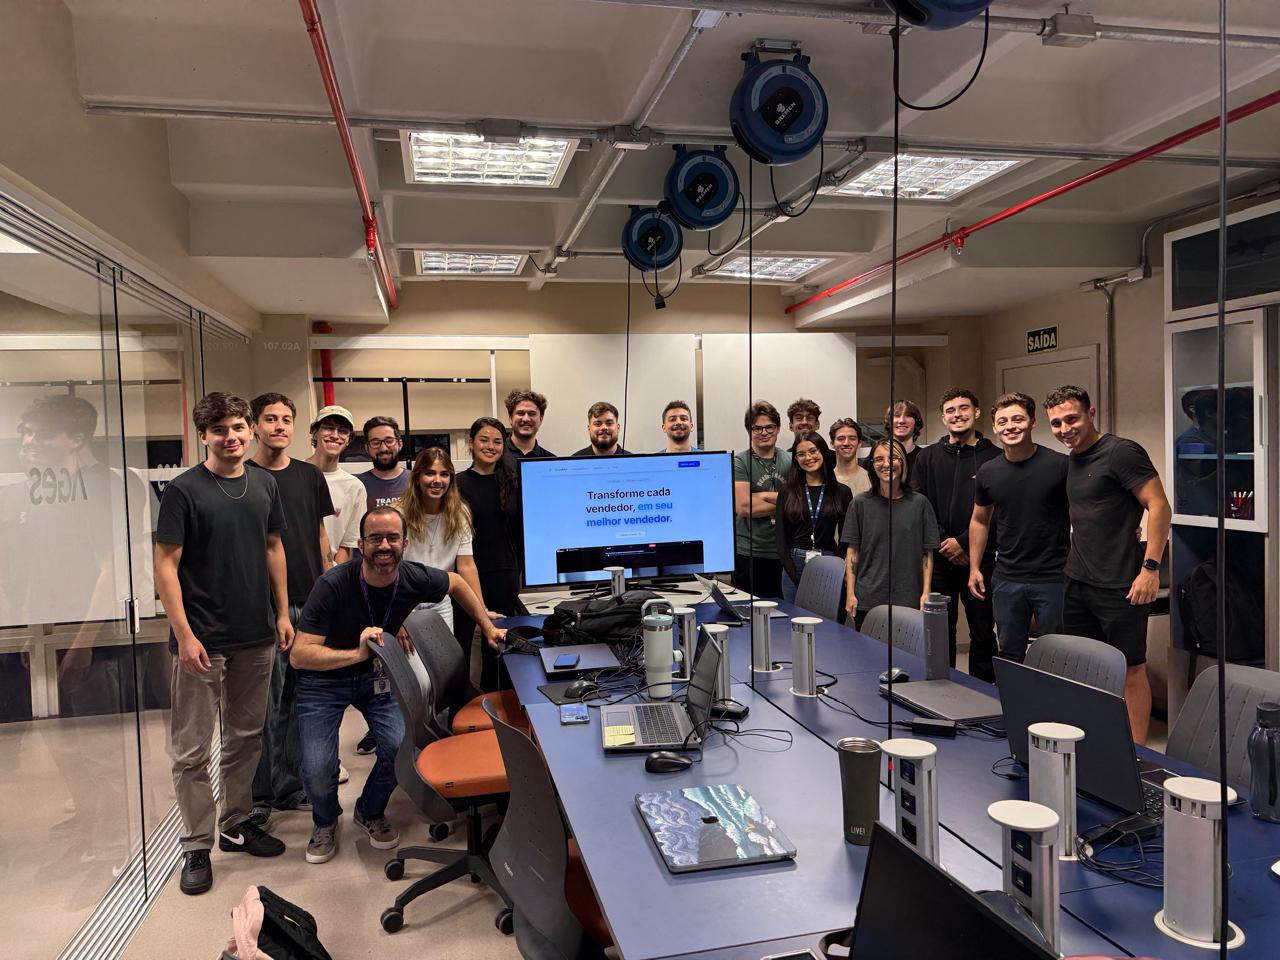
\includegraphics[width=1\linewidth]{conteudo/4 - ages III/conteudo/figures/foto-do-time.jpeg}
    \label{fig:projeto-time-sp}
    \href{https://tools.ages.pucrs.br/salespilot/wiki/-/wikis/home}{\textit{Fonte: https://tools.ages.pucrs.br/salespilot/wiki/-/wikis/home}}
\end{figure}

\begin{figure}[H]
    \centering
    \small
    \caption{Tela de detalhe de reunião com os \textit{insights} gerados pela IA}
    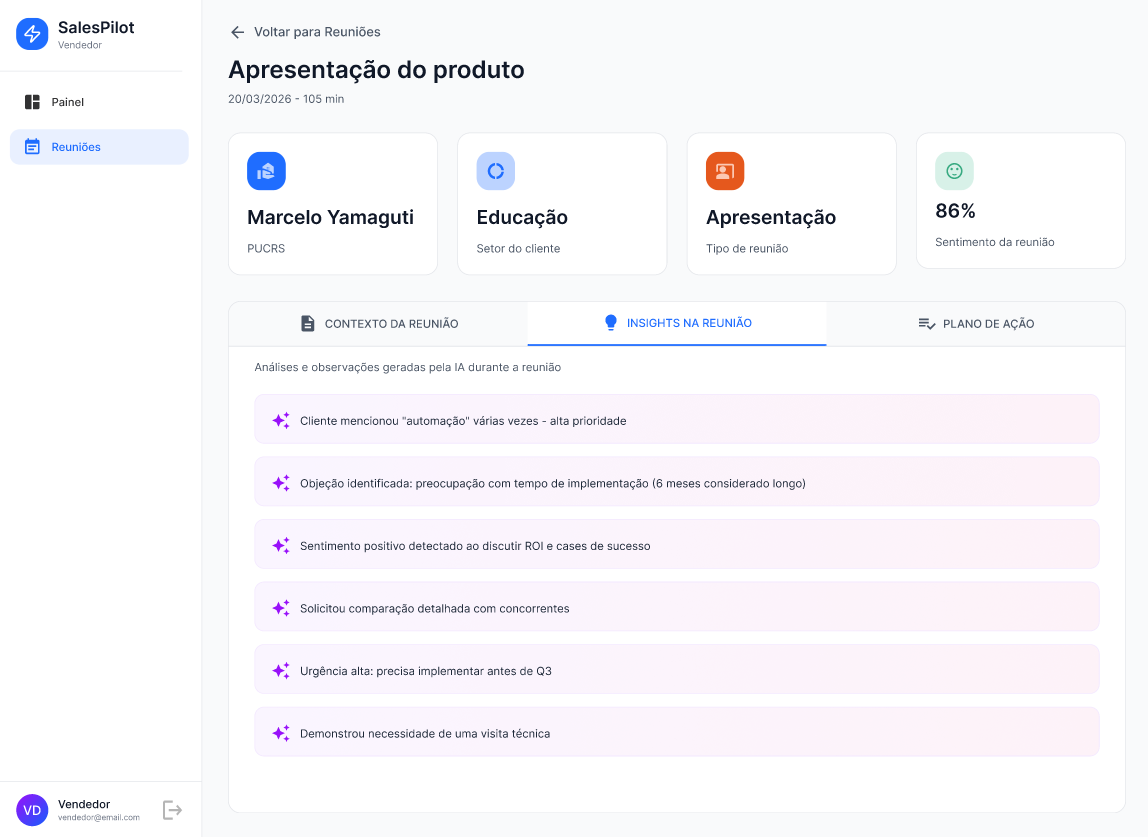
\includegraphics[width=0.7\linewidth]{conteudo/4 - ages III/conteudo/figures/meetings_insights_mockup.png}\\
    \label{fig:meetings-insights-mockup}
    \href{https://tools.ages.pucrs.br/salespilot/wiki/-/wikis/Design-Mockups}{\textit{Fonte: https://tools.ages.pucrs.br/salespilot/wiki/-/wikis/Design-Mockups}}
\end{figure}